\pagebreak
\chapter{Classification Results}
\label{sec:classifier}

\section{Data Analysis - Results}

\subsection{Results - Chunks per Subject}

t-test, maybe effect size, mention variance difference between groups and if they follow normal distribution

\subsection{Results - Subject Outliers}
\label{subs:res_outliers}

\begin{figure}[htbp]
 	\centering
	\begin{subfigure}{0.49\textwidth}
		\centering
		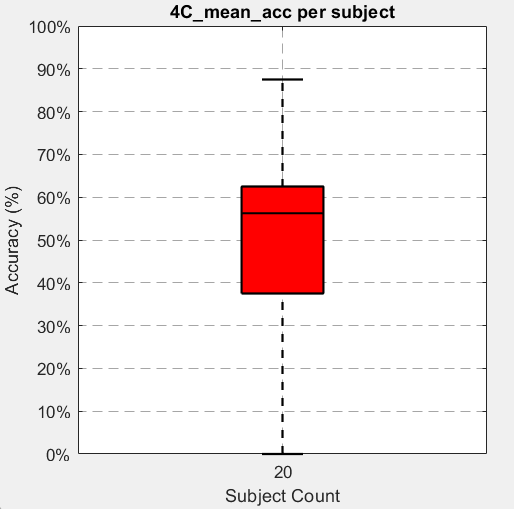
\includegraphics[width = 0.8\textwidth, height = 5cm]{assets/images/per_subj_4C_all.png}
		\caption{Boxplot illustating the initial spread of accuracies across individual subjects.}
		\label{fig:per_subj_all}
	\end{subfigure}
	\hfill
	\begin{subfigure}{0.49\textwidth}
		\centering
	 	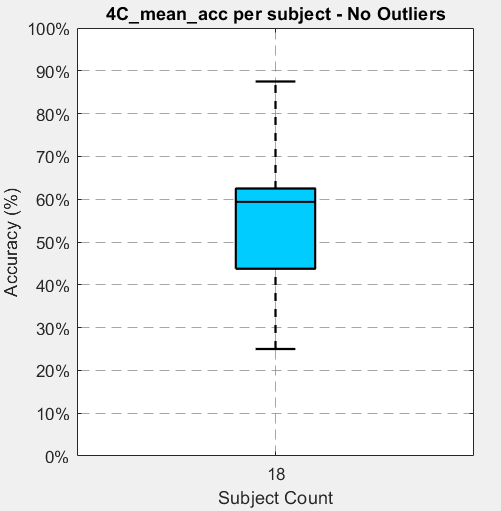
\includegraphics[width = 0.8\textwidth, height = 5cm]{assets/images/per_subj_4C_18.png}
		\caption{Boxplot illustating accuracy variance across individual subjects. after outliers have been excluded.}
		\label{fig:per_subj_18}
	\end{subfigure}
	\caption[Boxplots of Individual Subjects' Accuracies]{Boxplots produced during the "per subject" analysis.}
 	\label{fig:per_subj}
\end{figure}

After the classifier ran on each subject's data separately, using the maximum number of folds (4), the mean accuracies for each subject were calculated. As expected, these accuracies were generally lower than those obtained when the classifier was fed larger datasets. When all 20 subjects were included, the mean accuracy was 50\%, with a median value of 56.3\% (see figure \autoref{fig_per_subj_all}). However, two cases stood out immediately: Subject 100408 had a surprising accuracy of 0\%, and Subject 116524 showed an accuracy of 6.25\%. Given that the classifier completely failed to identify category-specific neural patterns in these subjects' data, it was assumed that the data was faulty for this analysis, and these subjects were excluded.

Once these outliers were removed, the mean accuracy for analyses involving one subject at a time increased to 55\%, with the median approaching 59.3\% (see figure \autoref{fig:per_subj_18}). Normally, this was still lower than the classifier's maximum potential accuracy of 61.9\%, which can be attributed to the low fold count used in these analyses. These results clearly indicate that screening for outlier subjects is crucial, as their inclusion can significantly impact the classifier's performance, particularly when working with smaller subject pools.

\subsection{Results - Fold Count}

The initial analysis, which focused on high fold counts, showed that accuracy stabilized to the second decimal point by 250 folds for both \gls{4C} and \gls{2C} analyses. This stability was reflected in the standard deviation of the distributions, which were 0.15\% for \gls{4C} and 0.17\% for \gls{2C}. In both cases, accuracy was slightly overestimated in the lower fold range of 250–1000, but eventually plateaued over 2500 folds, reaching 61.9\% for \gls{4C} and 70\% for \gls{2C}. These values represent the classifier's true accuracy and serve as the benchmarks to aim for in more practical, lower fold count analyses.

\begin{figure}[htbp]
 	\centering
	\begin{subfigure}{0.49\textwidth}
		\centering
		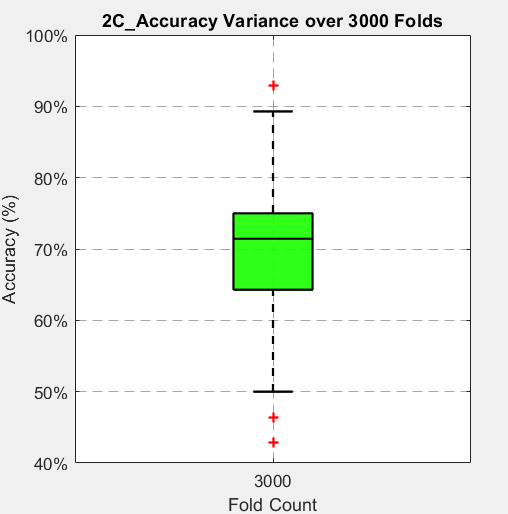
\includegraphics[width = 0.8\textwidth, height = 4cm]{assets/images/box_2C_3000.png}
		\caption{Accuracy variance across 3000 folds, for \gls{2C} data.}
		\label{fig:2C_3000}
	\end{subfigure}
	\hfill
	\begin{subfigure}{0.49\textwidth}
		\centering
	 	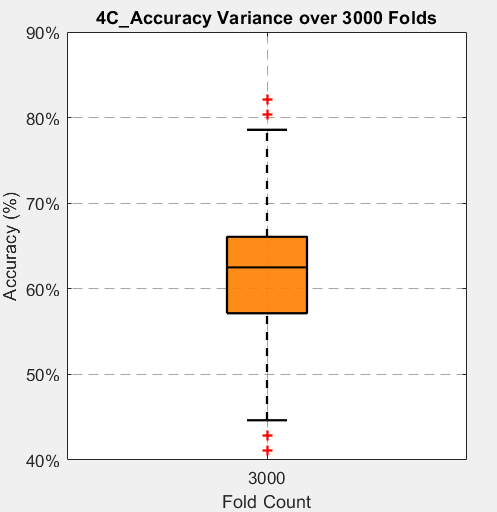
\includegraphics[width = 0.8\textwidth, height = 4cm]{assets/images/box_4C_3000.png}
		\caption{Accuracy variance across 3000 folds, for \gls{4C} data.}
		\label{fig:4C_3000}
	\end{subfigure}
	\caption[Boxplots of Accuracies across 3000 Folds]{Boxplots produced during the "high number of folds" analysis.}
 	\label{fig:fold_HN}
\end{figure}

Furthermore, figure \autoref{fig:fold_HN} presents a boxplot for both analyses, illustrating the spread of accuracies across all 3000 folds. This distribution of partitions drives the classifier to its benchmark performance. To establish a practical fold count, the partitioning scheme distribution should mimic the one shown in the boxplot. This rationale led to the optimal practical fold count values being set at 69 for \gls{2C} and 68 for \gls{4C}, as depicted in figure \autoref{fig:fold}.

\begin{figure}[htbp]
 	\centering
	\begin{subfigure}{0.49\textwidth}
		\centering
		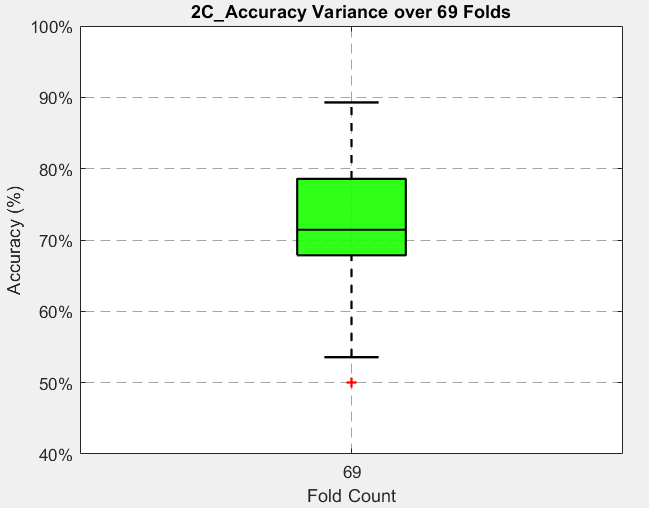
\includegraphics[width = 0.8\textwidth, height = 4cm]{assets/images/box_2C_69.png}
		\caption{Accuracy variance across the optimal 69 folds, for \gls{2C} data.}
		\label{fig:2C_69}
	\end{subfigure}
	\hfill
	\begin{subfigure}{0.49\textwidth}
		\centering
	 	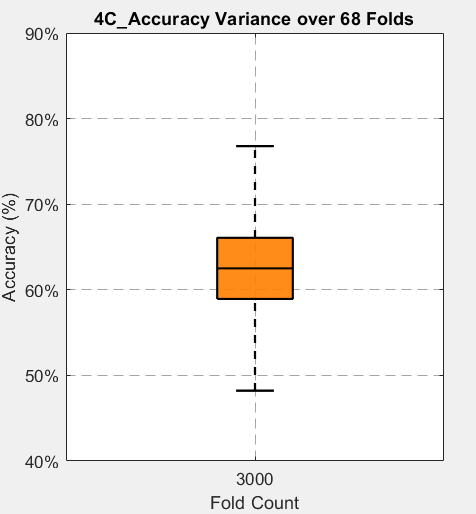
\includegraphics[width = 0.8\textwidth, height = 4cm]{assets/images/box_4C_68.png}
		\caption{Accuracy variance across the optimal 68 folds, for \gls{4C} data.}
		\label{fig:4C_68}
	\end{subfigure}
	\caption[Boxplots of Accuracies at optimal Fold Count]{The boxplots generated during the "practical fold count" analysis demonstrate distributions that closely resemble those obtained from the 3000-fold count analysis. These results indicate that the practical fold count approach provides both high accuracy and efficiency, making it a viable alternative for repeated analyses without compromising on the classifier's performance. The similarity in distributions confirms that reducing the number of folds to a more manageable level does not significantly affect the accuracy of the results.}
 	\label{fig:fold}
\end{figure}

\subsection{Results - Subject Count}

either trend line of data, extrapolte accuracy over 100+ subjects and when it stops being productive to gather more data [effect size(subject count)],
or, boxplot for every subject count and look at spread as well, plus median/mean trend line.

\subsection{Ideal Parameters Accuracy}

Optimal performance is achieved using, 2 chunks per run, 69 folds and 18 subjects. Accuracy is 72.3\%.